% Especificaciones del tamaño de letra, tamaño de hoja, márgenes, librerias, etc.
\documentclass[12pt, letterpaper]{article}
\usepackage[english]{babel}
\usepackage{fancyhdr}
\usepackage[utf8]{inputenc}
\usepackage[T1]{fontenc}
\usepackage{amsmath}
\usepackage{graphicx}
\usepackage{subcaption}
\usepackage[hidelinks]{hyperref}
\usepackage{url}
\usepackage{amssymb}
\usepackage{float}
\usepackage[margin=1in]{geometry}
\renewcommand{\baselinestretch}{1.5}

% Enlace Bibliografía
\usepackage{csquotes}
\usepackage[notes,backend=biber]{biblatex-chicago}
\addbibresource{referencias.bib}

% Titulo, autores, fecha.
\title{Homework \#1: Most Common Aircraft Engines}
\author{Carlos A. Vásquez Castañeda \and 1155057 \and Group 392}
\date{August 21, 2019}
\pagestyle{fancy}
\fancyhf{}
\rhead{Aircraft Elements Design}
\lhead{Homework \#1}
\rfoot{\thepage}


% Inicio del documento
\begin{document}
\maketitle
\section*{Introduction}
Motors have been studied exhaustively throughout the past. These operate under simple concepts and the many uses we've found for them has lead us to develop better technology over the last few decades. Not all of them are created in the same way nor with the same purpose, but there's such a huge list of them that it's impossible to imagine modern society without them.

In the aerospace industry, motors may vary depending on the circumstance and the purpose, but something's for sure, they ought to be trustworthy and tested thouroughly to assure proper functioning. We shall now proceed and anylize the most used motors in the industry.

\subsection*{Turbofan}
\subsubsection*{Description}
Also known as "fanjet" or "bypass engine", is an engine which produces thrust using a combination jet core efflux/jet blast and bypass air which has been accelerated by a ducted fan that is driven by the jet core.\autocite{skybrary16}
It is essentially a modern variation of the turbine engine and very similar to the turbojet.
\subsubsection*{Characteristics}
In a turbofan engine the core engine is surrounded by a fan in the front and an additional turbine in the rear and are connected to an additional shaft (Colored green in Figure 1.)
\begin{figure}[H]
	\centering
	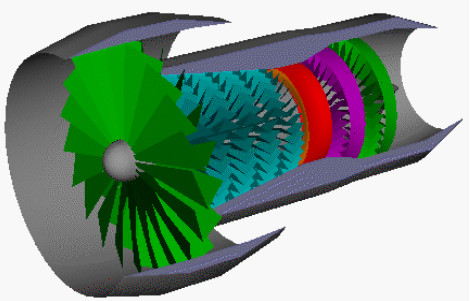
\includegraphics[width=0.5\textwidth]{1.png}
	\caption{General schematic of the turbofan engine.}
\end{figure}
As with the core compressor and turbine, some of the fan blades turn with the shaft and some remain stationary. This type of arrangement is called \textit{two-spool} engine (since the engine has two shafts, one "spool" for the fan, another "spool" for the core). More advanced engines have three-spools or higher, as the number of spools increases the efficency.

The most important characteristic of the turbofan is, when the air comes through the inlet, some of that air passes through the fan and continues on into the compressor and then the burner, where it's mixed with fuel and combustion occurs, but some of the air bypasses the engine itself just like the air through a propeller. This way a turbofan gets some of its thrust from the core and some from its thrust from the fan. With these engines, an important ratio, called the \textit{bypass ratio} is to be determined in order to determine the efficency. It is defined as the ratio of air that goes around the engine to the air that goes through the core. \autocite{nasa00}
\subsubsection*{Is it still in use?}
The turbofan is still widely used by modern fight planes and commercial planes.
\subsubsection*{Examples}
\begin{figure}[H]
	\centering
	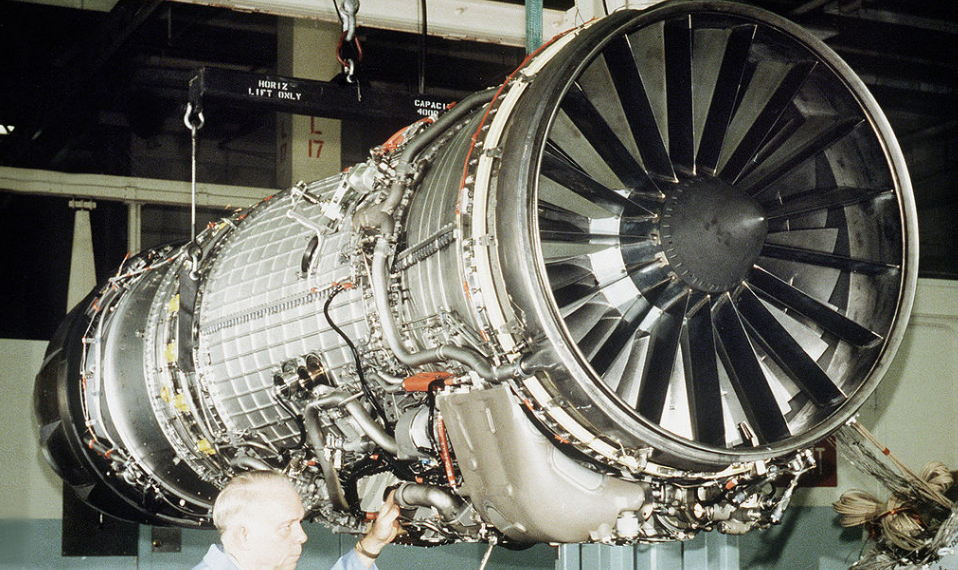
\includegraphics[width=0.5\textwidth]{2.png}
	\caption{General Electric F110 with low bypass ratio, used in fighter planes.}
\end{figure}

\subsection*{Turboprop}
\subsubsection*{Description}
Also known as "turbopropeller", it's commonly used in low speed transport aircraft and small commuter aircraft. It also relies heavily on the gas turbine engine as its basis and core to turn a propeller. Propeller engines develop thrust by moving a large mass of air through a small change in velocity. Propellers are very efficient.

The turboprop engine offers several advantages over other types of engines, such as being lightweight, having a great mechanical reliability due to relatively few moving parts, simplicity of operation, minimum vibration, high power per unit of weight, and being used for takeoff and landing.

Altough they offer many advantages, they become less efficient as the speed of the aircraft increases, turboprops are only used for low speed aircraft like cargo planes. They are more efficient at speeds between 250 and 400 mph and altitudes between 18,000 and 30,000 feet. \autocite{nasa01} \autocite{faa17}

\begin{figure}[H]
	\centering
	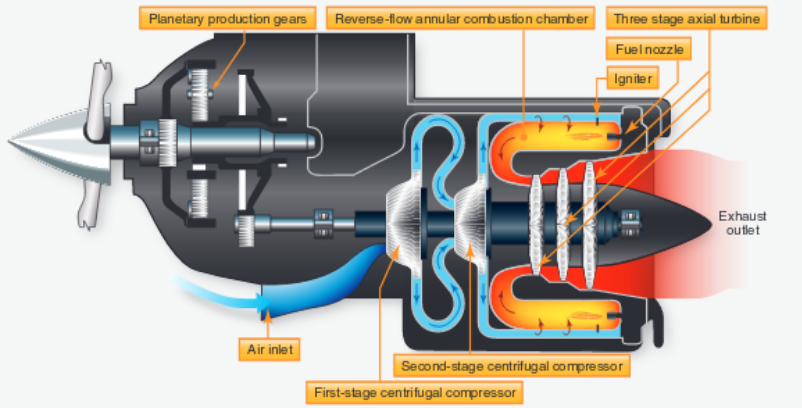
\includegraphics[width=0.8\textwidth]{3.png}
	\caption{General schematic of a fixed shaft turboprop engine.}
\end{figure}

\subsubsection*{Characteristics}
The turboprop has two main parts, the core and the propeller. The core is very similar to that of a basic turbojet or turbofan except that instead of expanding all the hot exhaust through the nozzle to produce thrust, most of the energy of the exhaust is used to turn the turbine. The drive shaft is connected to a \textit{gear box}. The gear box is connected to a propeller that produces most of the thrust.

As it was said in the last section, turboprops are really reliable when it comes to low speed aircraft, but when speed is a concern the turboprop won't have the means to compete with other engines.
\subsubsection*{Is it still in use?}
Yes. AS it has been said, they are primarily used for low speed. medium altitude aircrafts, like cargo planes.

\subsubsection*{Examples}
\begin{figure}[H]
	\centering
	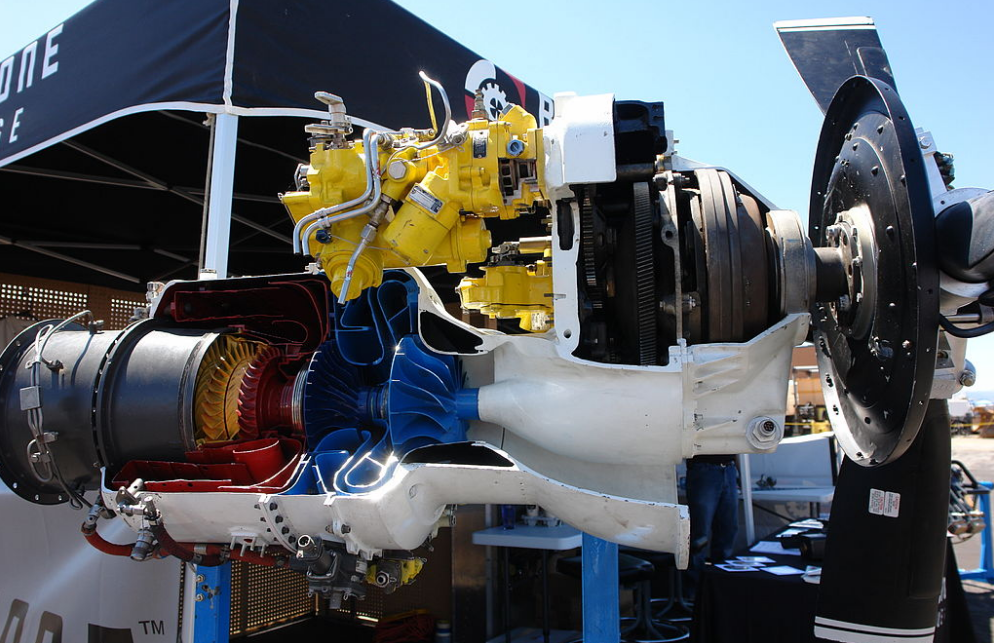
\includegraphics[width=0.7\textwidth]{4.png}
	\caption{Photo of a Garret TPE-331 turboprop engine.}
\end{figure}

\subsection*{Turbojet}

\subsubsection*{Description}
It is a jet engine, the simplest of them and the oldest too, in which a turbine-driven compressor draws in and compresses air, forcing it into a combustion chamber into which fuel is injected. Ignition causes the gases to expand and rush first through the turbine and then through the nozzle at the rear. Forward thrust is generated as a reaction to the rearward momentum of the exhaust gases.
The fist turbojet powered aircraft was a Heinkel He 178, which was flown in Germany in 1939.\autocite{britannica00}

\begin{figure}[H]
	\centering
	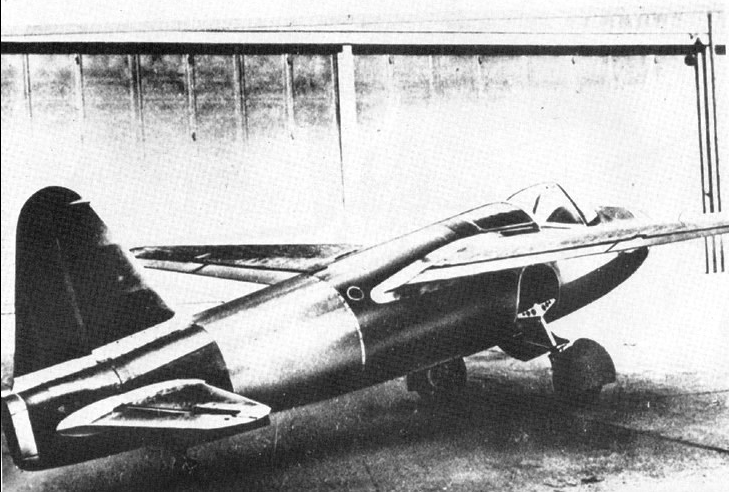
\includegraphics[width=0.5\textwidth]{5.png}
	\caption{Heinkel He 178}
\end{figure}
\subsubsection*{Characteristics}
The layout is basically the same as the turbofan, but instead of a two-spool design, the turbojet only has one shaft. Air is brought to the inlet (or intake), then it goes through the compressor which changes the pressure of the air flowing through it. Afterwards the air arrives at the burner and a small amount of fuel is added and ignited. The hot air and gases finally go through the turbine, which extracts the energy from the hot gases and with it turns the compressor. This is done by linking the compressor and the turbine with a central shaft.\autocite{nasa02}
\begin{figure}[H]
	\centering
	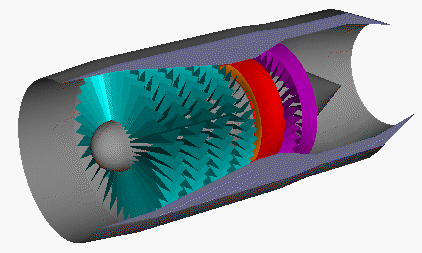
\includegraphics[width=0.6\textwidth]{6.png}
	\caption{General schematic of a turbojet engine.}
\end{figure}
\subsubsection*{Is it still in use?}
It's true that turbofans are more widely used nowadays but turbojets have their uses too which can vary from carrying passenger to cargo and military aircraft. Also a lot of private airplanes use these.
\subsubsection*{Examples}
\begin{figure}[H]
	\centering
	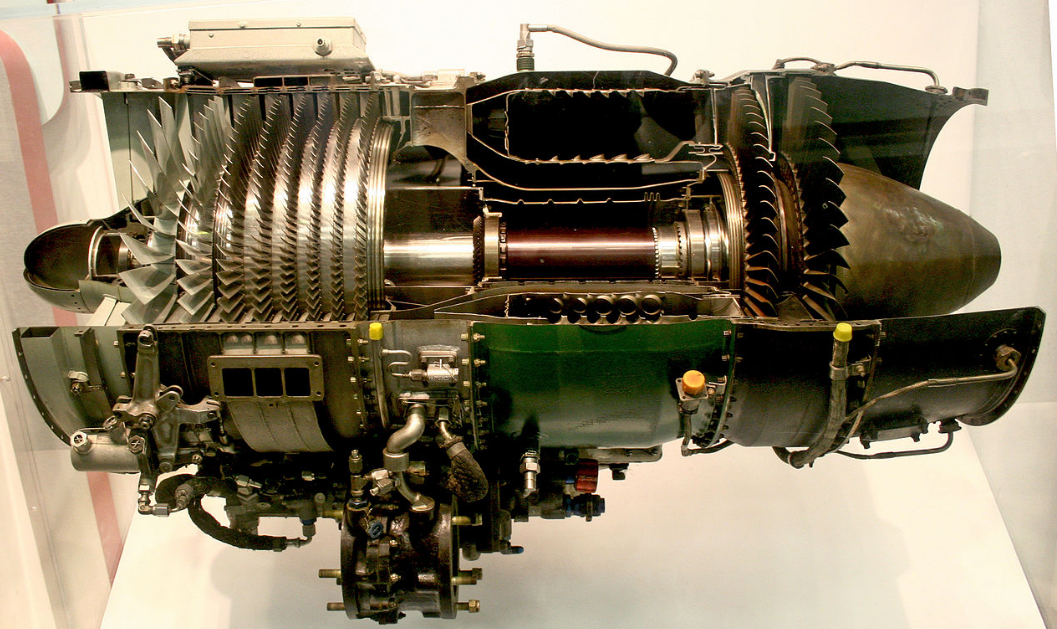
\includegraphics[width=0.6\textwidth]{7.png}
	\caption{J85-GE-17A, turbojet engine made by General Electric in 1970.}
\end{figure}

\subsection*{Turboshaft}

\subsubsection*{Description}
Turboshafts are engines similar to turbopropellers. One of the main features of these engines is their ability to takeoff and land vertically, and so their use where area is limited is invaluable such as emergency rescue services. Widely used by helicopters and hovercraft.\autocite{pbs00}

\subsubsection*{Characteristics}
A turbo shaft engine is a form of gas turbine which is optimized to produce shaft power, rather than jet thrust. It has additional turbine expansion to extract heat energy from the exhaust and convert it into output shaft power.
The general layout of a turboshaft is similar to that of a turboprop. The main difference is a turboprop is structurally designed to support the loads created by a rotating propeller, as the propeller is not attached to anything but the engine itself. In contrast, turboshaft engines usually drive a transmission which is not structurally attached to the engine. The transmission is attached to the vehicle structure and supports the loads created instead of the engine.
\begin{figure}[H]
	\centering
	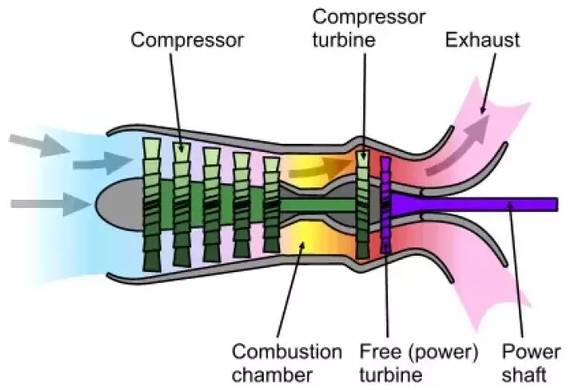
\includegraphics[width=0.6\textwidth]{8.png}
	\caption{General schematic of a turboshaft engine.}
\end{figure}
\subsubsection*{Is it still in use?}
Widely used nowadays in hover aircraft, helicopters, tanks, boats and ships.

\subsubsection*{Examples}
\begin{figure}[H]
	\centering
	
\includegraphics[width=0.6\textwidth]{9.png}
	\caption{The T901 turboshaft by General Electric, made for military purposes.}
\end{figure}

\subsection*{RAT}

\subsubsection*{Description}
A ram air turbine (RAT) is a small, windmill-like device that is deployed into the airstreams flowing around the aircraft. Modern aircraft have an additional power system called the auxiliary power unit (APU) which can take over responsibility for the hydraulic system in an emergency, however, the APU is itself a small engine, and needs fuel in order to operate. If the airplane loses its fuel, neither engines nor the APU can keep the airplane in a controllable state. The RAT solves this issue. 
\subsubsection*{Characteristics}
It converts a small portion of the energy in the flow into hydraulic and/or electrical power for the aircraft, allowing it to be flown even if the plane is entirely empty of fuel. \autocite{wt08}
In case of an all engine failure, the RAT is deployed to generate electric/hydraulic required for the operation of critical instruments. As the airplane moves (gliding in case of engine failure) the relative airflow rotates the leafs of RAT, which is coupled to an electric generator/hydraulic motor.
\subsubsection*{Is it still in use?}
It is still used, specially in military and commercial aircraft where safety is priority.
\subsubsection*{Examples}
\begin{figure}[H]
	\centering
	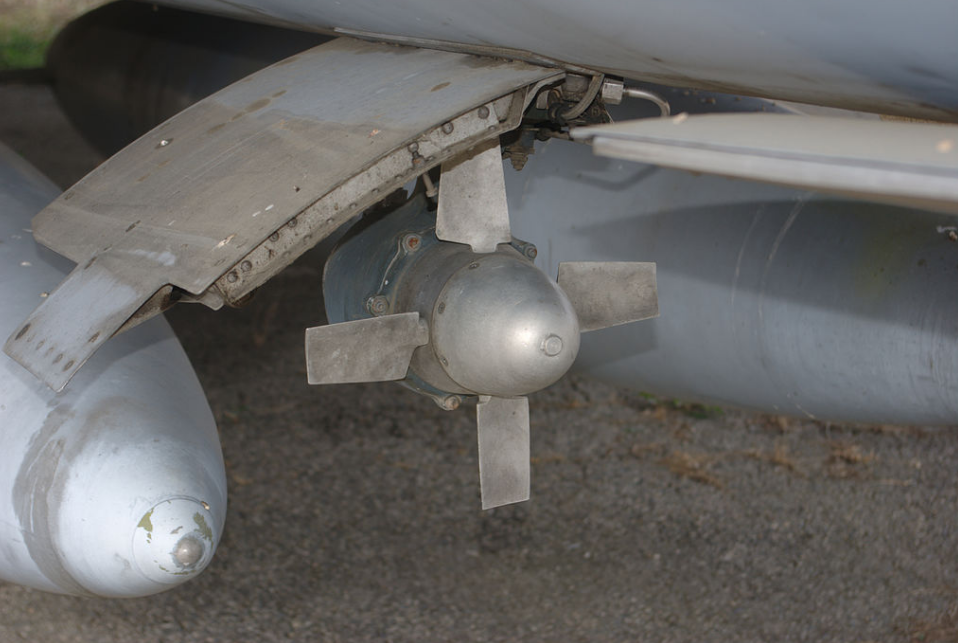
\includegraphics[width=0.6\textwidth]{10.png}
	\caption{RAT from swedish aircraft Saab 35 Draken.}
\end{figure}

\subsection*{APU}

\subsubsection*{Description}
An Auxiliary Power Unit or APU allows an aircraft to operate autonomously without reliance on ground support equipment such as a ground power unit, an external air-conditioning unit or a high pressure air start cart. They serve as a source of electrical power before the main aircraft engines begin to run. They supply electrical power to onboard networks, especially for starting the main engines or for supplying onboard devices and air conditioning units.\autocite{skybrary17} \autocite{pbs01}

\subsubsection*{Characteristics}
The APU is essentially a small jet engine consisting of a two-stage centrifugal compressor directly coupled to a single-stage inward flow turbine. The APU is normally located in the tail cone of the aircraft but, in some cases, is located in an engine nacelle or in the wheel well.
\begin{figure}[H]
	\centering
	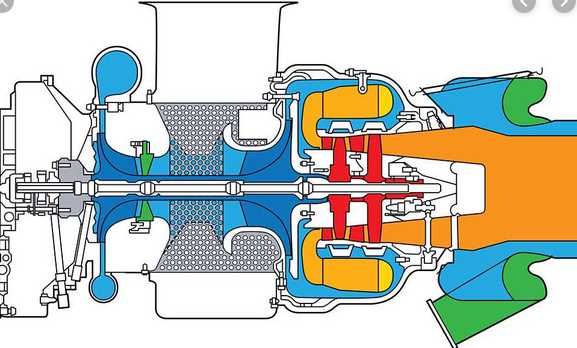
\includegraphics[width=0.6\textwidth]{11.png}
	\caption{Schematic of an APU.}
\end{figure}
\subsubsection*{Aún se utiliza}
Used in commercial and private aircraft.
\subsubsection*{Examples}
\begin{figure}[H]
	\centering
	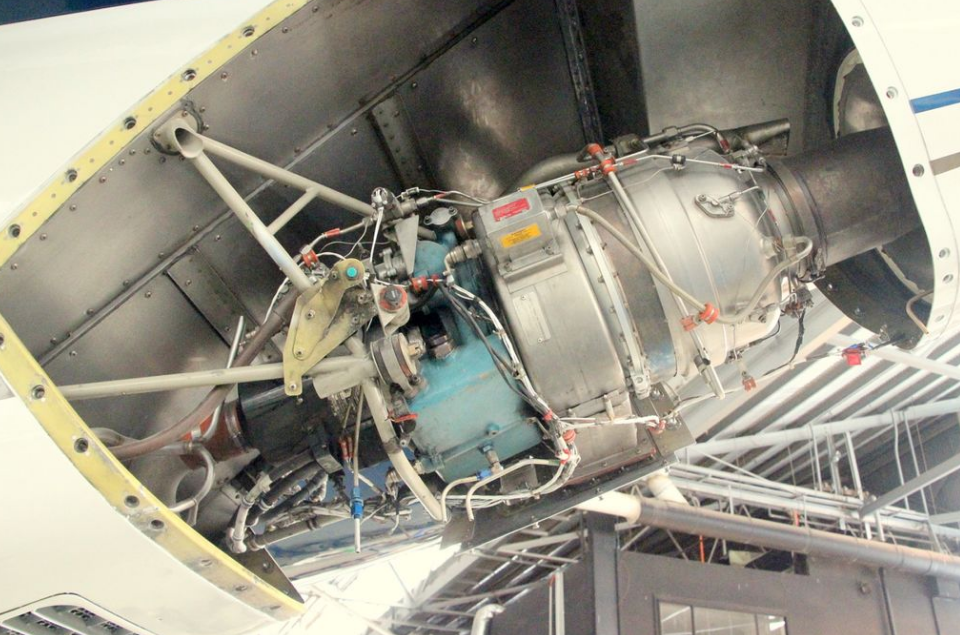
\includegraphics[width=0.6\textwidth]{12.png}
	\caption{A Honeywell GTCP36 APU mounted under the tail of a business jet.}
\end{figure}
%%%%%  Bib
\renewcommand\refname{References}
\printbibliography
\end{document}
